%\newtheorem{definition}[subsection]{Definition}
%\newtheorem{example}[subsection]{Example}
\newtheorem{cor}[subsection]{Corollary}
\newtheorem{pro}[subsection]{Proposition}
\newtheorem{theo}[subsection]{Theorem}
\newtheorem{lem}[subsection]{Lemma}
%\newtheorem{rem}[subsection]{Remark}

\definecolor{main}{HTML}{5989cf}    % setting main color to be used
\definecolor{sub}{HTML}{cde4ff}     % setting sub color to be used

\tcbset{
    sharp corners,
    colback = white,
    before skip = 0.2cm,    % add extra space before the box
    after skip = 0.5cm      % add extra space after the box
}                           % setting global options for tcolorbox

% You can copy any following box you like to your code.
\newtcolorbox{boxA}{
    fontupper = \bf,
    boxrule = 1.5pt,
    colframe = black % frame color
}

\newtcolorbox{boxB}{
    fontupper = \bf\color{main}, % font color
    boxrule = 1.5pt,
    colframe = main,
    rounded corners,
    arc = 5pt   % corners roundness
}
\newtcolorbox{boxC}{
    colback = sub, % background color
    boxrule = 0pt  % no borders
}

\newtcolorbox{boxD}{
    colback = sub, 
    colframe = main, 
    boxrule = 0pt, 
    toprule = 3pt, % top rule weight
    bottomrule = 3pt % bottom rule weight
}

\hypersetup{
    colorlinks=true,
    linkcolor=blue,
    filecolor=magenta,      
    urlcolor=cyan,
    pdftitle={Overleaf Example},
    pdfpagemode=FullScreen,
    }

\urlstyle{same}



\coursetitle{\mtthreeiii}{MT303}%\coursetitle{\mtthreeiii}{MT303}
\developers{  Wyclife Rao }
\reviewers{Dr Irene Sitawa }
\modulenumber{0}

\modulename{STACK Syntax}

% courses
\thispagestyle{empty}
\begin{tikzpicture}[overlay,remember picture,font=\sffamily\bfseries]
 \draw[ultra thick,c4,name path=big arc] ([xshift=-2mm]current page.north) arc(150:285:11) coordinate[pos=0.225] (x0);
 \begin{scope}
  \clip ([xshift=-2mm]current page.north) arc(150:285:11) --(current page.north east);
  \fill[c4!50,opacity=0.25] ([xshift=4.55cm]x0) circle (4.55);
  \fill[c4!50,opacity=0.25] ([xshift=3.4cm]x0) circle (3.4);
  \fill[c4!50,opacity=0.25] ([xshift=2.25cm]x0) circle (2.25);
  \draw[ultra thick,c4!50] (x0) arc(-90:30:6.5);
  \draw[ultra thick,c4] (x0) arc(90:-30:8.75);
  \draw[ultra thick,c4!50,name path=arc1] (x0) arc(90:-90:4.675);
  \draw[ultra thick,c4!50] (x0) arc(90:-90:2.875);
  \path[name intersections={of=big arc and arc1,by=x1}];
  \draw[ultra thick,c4,name path=arc2] (x1) arc(135:-20:4.75);
  \draw[ultra thick,c4!50] (x1) arc(135:-20:8.75);
  \path[name intersections={of=big arc and arc2,by={aux,x2}}];
  \draw[ultra thick,c4!50] (x2) arc(180:50:2.25);
 \end{scope} 
 \path[decoration={text along path,text color=c4,
                 raise = -2.8ex,
                 text  along path,
                 text = {},%|\sffamily\bfseries|02/18/2019
                 text align = center,
             },
             decorate
         ] ([xshift=-2mm]current page.north) arc(150:245:11);
 %
 \newcommand\add{4cm}
 \begin{scope}%[shift={(5,0)}]
  \path[clip,postaction={fill=c3}]
  ([xshift=2cm+\add,yshift=-8cm]current page.center) rectangle ++ (4.6,7.7);
  \draw[c5,ultra thick,fill=c2] ([xshift=0.5cm+\add,yshift=-8cm]current page.center)
   ([xshift=0.5cm+\add,yshift=-8cm]current page.center)  arc(180:60:2)
    |- ++ (-3,6) --cycle;
  \draw[ultra thick,c5] ([xshift=-1.5cm+\add,yshift=-8cm]current page.center) 
  arc(180:0:2);
  \draw[ultra thick,c5] ([xshift=0.5cm+\add,yshift=-8cm]current page.center) 
  arc(180:0:2);
  \draw[ultra thick,c5] ([xshift=2.5cm+\add,yshift=-8cm]current page.center) 
  arc(180:0:2);
  \draw[ultra thick,c5] ([xshift=4.5cm+\add,yshift=-8cm]current page.center) 
  arc(180:0:2);
  \fill[white] ([xshift=2.5cm+\add,yshift=-8cm]current page.center) +(60:2) circle(1.5mm)
  node[above
  right=0mm,text=c5!80!black]{$\rho:=\dfrac{1+\sqrt{-3}}{2}$};
 \end{scope}
 %
 \fill[c1] ([xshift=2cm+\add,yshift=-8cm]current page.center) rectangle ++ (-30.7,7.7);
 \node[text=white,anchor=west,scale=2.3,inner sep=0pt] at
 ([xshift=-10cm,yshift=-1.8cm]current page.center) {\color{ulabgold} LEARNING};
 \node[text=white,anchor=west,scale=5,inner sep=0pt] at
 ([xshift=-10cm,yshift=-3.25cm]current page.center) {MODULE \dpmdnumber};
 \node[text=white,anchor=west,scale=2.5,inner sep=0pt,text width=.4\textwidth] at
 ([xshift=-10cm,yshift=-6cm]current page.center) {\dpmdname};
 \node[text=white,anchor=east,scale=2,inner sep=0pt] at
 ([xshift=5.7cm,yshift=-7.5cm]current page.center) {\color{ulabgold}The Open University of Kenya};
 %
% \draw[gray,line width=5mm] 
% ([xshift=2mm,yshift=-1mm]current page.south west) rectangle ([xshift=-2mm,yshift=1mm]current
% page.north east);
\end{tikzpicture}

%\newpage
\pagenumbering{roman}
\thispagestyle{empty}%firstpage


\begin{center}
\vspace*{2cm}
{\Huge\bf BACHELOR OF TECHNOLOGY EDUCATION}\\[3cm]  


%{\fontsize{80}{40}\selectfont \dpcoursecode}\\[2cm]
%
%{\fontsize{30}{40} \selectfont \dpcoursename}\\[2cm]

%\rule{\textwidth}{1pt}
%\vspace{2cm}

%{\fontsize{40}{40}\selectfont \bf Module~\dpmdnumber}\\[2cm]
%
%{\fontsize{30}{40}\selectfont \bf \dpmdname}\\

\vfill
\begin{flushright}
\begin{minipage}{.6\textwidth}
\begin{tcolorbox}%[text ]
\begin{tabular}{ll}%\hline
\subtitle{Developed by:}&\displaydevelopers\\
&\\
\subtitle{Reviewed by:}&\makecell[l]{\displayreviewers}\\
\end{tabular}
\end{tcolorbox}
\end{minipage}\hspace*{-3.5cm}
\end{flushright}
\vspace*{-2.5cm}
\end{center}

\newpage
\thispagestyle{empty}
\null
\vfill
{\renewcommand\arraystretch{1.5}
\begin{tabular}{|l|l|}\hline
\subtitle{Programme Title} & Bachelor of Technology Education \\\hline
\subtitle{Course Title} & \fullcoursename\\\hline
\subtitle{Learning Module number} & Module \dpmdnumber\\\hline
\subtitle{Learning module title} & \dpmdname \\\hline
\subtitle{Module Developer} & \displaydevelopers\\\hline
\subtitle{Reviewed by} & \displayreviewers\\\hline
%\subtitle{Vision} & \vision\\\hline
%\subtitle{Audience description} & \\\hline
\end{tabular}}
\clearpage
%\section{COURSE LEARNING GUIDE}


\subsection*{Preparing for Online and Distance Learning}

This course offers you the opportunity to enter an online space where you can engage with fellow students at the university. The online forums, exercises, tasks and materials have been designed by the course facilitators in such a way that you can draw directly from their knowledge and share in their scholarly interest in online learning and assessment

We hope you will use your access to this virtual classroom to raise all your questions on the course module, to build a network great learners and to share your own thoughts and experiences to the benefit of your fellow students.

   
There are a number of steps you can take to ensure you are well prepared to make the most of this learning opportunity. This resource should prompt you to consider the following:


 \begin{enumerate}[label=\cb$\square$]
   \item How can you best prepare the space where you expect you will spend most of your time engaging in online learning (i.e. in your home or office, or even during your commute to work or whilst traveling)?
  \item   What can you do to ensure you keep working through the course material, even when you do not have Internet access?
    \item How can you familiarise yourself with the course layout, in order to be able to navigate through the steps with ease?
    \item What are the communication strategies and best practices you could consider to best engage with your fellow students and the course facilitators?
    \item What do you do when you need academic or technical support?

 \end{enumerate} 

\subsection*{General Module Guide}

The authors of this module believe that imparting knowledge should always be a mutual relationship between the students and the teachers. Students can actively construct knowledge through experiences gained in reading and answering the learning modules.

You should take time to read everything written in the module, actively and religiously solve all the exercises included to finish this course and be able to gain all the competencies and skills expected to demonstrate the learning outcomes as stated in this course. If you finish with full confidence that you understand and can apply all the knowledge you gain in this course, then you are sure to succeed in tackling the next higher subjects in your chosen course.

In this course, you will be taught not only the knowledge you need to demonstrate your learning outcomes, but you will also gain discipline, perseverance, higher thinking skills, and resourcefulness that would help strengthen your foundation to succeed in life. To successfully finish the course, you must follow the guides set forth in using this module.


\begin{description}[{format=\textcolor{ulabblue}}]
\item[STUDY ENVIRONMENT.]\leavevmode\\
Before engaging into the module, make sure that you are comfortable enough and diminish distractions. Make sure that you develop a study routine to perform and accomplish all the activities set forth by the module.
%\newpage

\item[MODE OF DELIVERY.]\leavevmode\\
Students are required to get a access a digitised copy of the module from the Virtue Learning Environment. As an open and distance learner, you should be able to learn independently and optimise the learning modes and environment available to you as much of  the delivery of all the lessons will be done asynchronously. Your success will greatly depend on your self-motivation and discipline to get your work done without your instructor to remind you from time to time.

\item[STUDY SCHEDULE.] \leavevmode\\
Remember that you have other subjects to attend to, hence, you must manage your time so that you will not be left behind in any of them. Create your own learning plan for each course to make sure that you can perform all the activities. Do not procrastinate your work, remember that time wasted can never be retrieved back. Make sure that even if you are at home, you are a student enrolled in a program, where the learning of all its courses greatly depends on your will to learn as the materials you need are all in your hands. So always be aware of your daily tasks.

\item[PRACTICE EXERCISE.]\leavevmode\\
To measure your learning from your reading, you are given practice exercises which you are supposed to answer daily. This will prepare you in performing your main task.

\item[ONLINE GROUP CHAT.]\leavevmode\\
I am going to create an online Discussion Forum and QA Forum  on the VLE.  This will serve as a room for discussion on the topics and activities found in your module.

\item[RECOMMENDED REFERENCES FOR SUPPLEMENTARY READING.]\leavevmode\\
You are given links that you need to access online. These links are online references such as e-books, online activities, and tutorial videos of the topic. These are other references you can use to further understand the topic and gain additional knowledge and skills.

\item[MAIN TASK.]\leavevmode\\
You are given a task that will require you to apply the knowledge and skills you learned from the module. This can be a group or individual activity which will measure your higher order thinking skills you acquired throughout the topic.

\item[RUBRICS. ]\leavevmode\\
This is a tool to guide you in performing your main task. Through this, you will be able to know the specific indicators that should be found in your task. This is to assess your constructive behaviour towards your learning application. You will be rated according to a 4-point scale shown below.
\begin{center}
{\color{ulabgold} \bf 4 − Excellent\quad\quad   3 −Good\quad\quad    2 − Fair \quad\quad  1 −Poor}
\end{center}
\item[REFLECTIONS.]\leavevmode\\
Writing your reflection will be a passageway to express your experiential learning in using this module. In your honest recall, write everything that you think happened to you during your learning experience in this module. Use the guide questions below:
\begin{description}[{format=\textcolor{ulabblue}}]
\item[First paragraph. ]\leavevmode\\
How was your learning experience? Maybe you can consider describing the effect of the parts of the module (sequence, discussions, examples, practice exercises, online activities, and the main task) in your learning experience. You can point out the strength and weakness of each part so that we can consider it for future improvement of this instructional material.
\item[Second paragraph.  ]\leavevmode\\
What did you learn? Did you successfully acquire the learning outcomes?

\item[Third paragraph.]\leavevmode\\
How can you use what you learned in the future?
\end{description}
\end{description}

\section{ASSESSMENT  TASKS \& EXAMINATION   RULES AND GUIDELINES}

\begin{enumerate}[label=\cb\arabic*.]
\item {\cb SUBMISSION OF ASSESSMENT TASTS.}

Since mathematical skills are best acquired through constant practice, you are encouraged to answer at least two (2) exercises a day. These practice exercises will not be graded but it will help you develop your thinking skills which will prepare you in the performance of your main tasks. You are required to submit your practice exercises every week.
\begin{center} {\cg Usually submission deadlines are set on Saturday 11:59PM EAT} \end{center}

\item  {\cb GROUP CHAT.}

You can post questions, solutions, and comment to other's post. Please be reminded that our group chat is exclusive only for discussion on topics related to this course. Everyone is required to actively participate in the discussions. Also, trolling is highly discouraged. Always observe proper online etiquettes when participating in discussions.
\begin{center} {\cb RULE OF THUMB: ALWAYS THINK BEFORE YOU CLICK} \end{center}

\item  {\cb MAIN TASK. }

Complete documentation during the preparation of your task is required to ensure that every member of the group participated and contributed in the task. May it be photos or screenshots of your virtual meetings or group works. You are going to submit it as attachment of your main task the same way as the practice exercises.



\item {\cb RECOMMENDED REFERENCES FOR SUPPLEMENTARY READING.} 

You can explore online for other references that is related to the topic to gain additional information about the topic. Do not share or post inappropriate materials online or even privately.
\end{enumerate}

\subsection*{Requirements to pass the course}

Compiled Continuous  Assignment/Activities and Tasks  with Final Performance Examination.

\subtitle{Grading System}
\begin{center}
{\renewcommand\arraystretch{1.5}
\begin{tabular}{|l|c|}\hline
Continuous Activities and Tasks  &  50\%\\\hline
Final Performance Examination. &  50\%\\\hline
\end{tabular}
}
\end{center}
%\newpage










%\subsection{INTRODUCTORY MESSAGE}

%A warm welcome to \;  \fullcoursename, {\bf Module on \dpmdname}.



%By this module learning resource, we aim to enable you  achieve the relevant competencies, depict skill, action and purpose successfully. 
 

%It has been designed to provide you with fun and meaningful opportunities for guided and independent learning at your own pace and time. You will be enabled to process the contents of the learning material while being an active learner. Your academic success lies in your own hands.  This module has the following parts and corresponding icons:





{
\renewcommand\arraystretch{4}
\begin{longtblr}{
width=\linewidth,
 colspec={ Q[1,c,f] Q[1.5,r,m] Q[4,l,m] },
%row{1} = { font=\bfseries },
% rowhead = 1,
  caption={ }, 
  label={ },
  rowsep = 4pt,
  hlines = {ulabblue!20, 1pt},
  vlines = {ulabblue!20, 1pt},
}

\includegraphics[width=2cm]{img/audience} & {\bf AUDIENCE}  &  This is a description of a target audience.   \\
{\fontsize{40}{30}\selectfont\color{ulabblue}\faCogs}& {\bf MODULE DESCRIPTION} & 
This part explains the importance of the topics discussed in the module. It will also give you a sneak peek of what you will learn and what is expected from you at the end of the module.\\

\includegraphics[width=2cm]{img/target.png} &  {\bf  EXPECTATION} & These are what you will be able to know after completing the lessons in the module\\

\includegraphics[width=2cm]{img/preactivities} & {\bf PRE-ACTIVITY} &
This activity is to get you set, activate and engage schema to learn the module. Through this activity, you will know the relevance of this activity to the topic that will be discussed in the module.\\

\includegraphics[width=2cm]{img/pretest} &  {\bf PRE - ASSESSMENT} & This will measure your prior knowledge and the concepts to be mastered throughout the lesson. \\

\includegraphics[width=1.7cm]{img/rewind} &  {\bf  RECAP} & This section will measure what learnings and skills that you understand from the previous lesson.\\

\includegraphics[width=1.5cm]{img/lesson} &  {\bf  LESSON} & This section will discuss the topic for this module.\\

\includegraphics[width=2cm]{img/activities} &  {\bf  ACTIVITIES} & This is a set of activities you will perform.\\

\includegraphics[width=2cm]{img/summary} &  {\bf  WRAP UP} & This section summarizes the concepts and applications of the lessons.\\

\includegraphics[width=2cm]{img/discussion}& {\bf DISCUSSIONS} &
This is the meat of the module. The discussion is aligned to the topic learning outcomes that is expected of you to acquire at the end of the module.\\

\includegraphics[width=1.8cm]{img/value} &  {\bf  VALUING} & This part will check the integration of values in the learning competency you will take home.\\

\includegraphics[width=1.8cm]{img/posttest} &  {\bf  POST - ASSESSMENT} & This will measure how much you have learned from the entire module.\\

\includegraphics[width=1.8cm]{img/selfreflect} & {\bf REFLECTION }
&
This part is for you to share your thoughts by writing your reflection, make sure to check your grammar and spelling to ensure the readability and so that it will not alter the thought being delivered. 
\end{longtblr}
}









%\vfill

\audience
\begin{oldactivity}{Audience Description}{
\includegraphics[width=22mm]{img/audience}}{}
This module is offered to all students taking the Bachelor of Technology Education. As an open and distance learner, you should be able to learn independently and optimise the learning modes and environment available to you. Before you begin this course, please confirm the course material, the course requirements and how the course is conducted.
\end{oldactivity}
%\newpage
\pagenumbering{arabic}



\mddescription
In this module you are carried through the syntax used in keying in responses in STACK.
%\begin{itemize}
%\item round-off errors and computer arithmetic
%\item algorithms in numerical computation 
%\item convergence of iterative processes
%\item solutions of equations of one variable using bisection method, fixed point iteration and Newton's method
%\end{itemize}

%\expectations
%\begin{enumerate}
%\item define functions of several variables, graphs of functions of several variables, level curves.
%\item relate the above terminologies to real life situations.
%\item solve problems involving functions of two variables with regard to determining their domain, graphs, level curves.
%\item relate concepts of functions of several variables to real life situations; topographic map of a mountain range, plot of sea level over time, graph of temperature versus altitude, plot of a stock's performance over a year, map of population density by country.
%\end{enumerate}


%\begin{mlos}
%\item Define round-off errors and identify their sources in numerical computations.
%\item explain the significance of algorithms and convergence of iterative techniques in numerical computations.
%  \item Use the bisection and Newton’s methods to find roots of nonlinear equations.
%  \item Compare the efficiency and convergence rates of bisection, fixed point iteration, and Newton’s methods
%\end{mlos}
%
%%tttttttttttttttttttttttttttttttttttttttttttttttttttttttttttttttttttttttttttttttttttttttttttttttttttttttttttttttttttttttttttttttttttttttttttttttt
%%\begin{large}{Module 1}\end{large}
%\section*{What and why numerical methods}
%\begin{youtube}[]
%For an introductory remark about numerical methods watch the \\videos whose links are provided.
%
%% and then attempt the subsequent quiz.
%\mylink{https://www.youtube.com/watch?v=IOR31yN43Kg}
%
%\mylink{https://www.youtube.com/watch?v=YjOsUQTJDpk}
%\end{youtube}
%
%%\begin{pretest}
%%
%%\item 
%%\end{pretest}
%
%%\begin{myexercise}\label{Comprehensionquiz2}
%%\begin{enumerate}[label=\arabic*.]
%%\item 
%%
%%\end{enumerate}
%%\end{myexercise}
%%
%%
%%{\bf The content of each of the following three sections is to be pre-recorded in videos which learners are to watch before attempting the comprehension quiz}
%
%\section{Computer Arithmetic and Round-off Errors}
%
%\videolesson
%\begin{selfvideo}[1]
%\comx{The following pre-recorded video discusses the concepts of computer arithmetic and round-off errors. Watch it and also go through the interactive content. Thereafter attempt the comprehension quiz that follows.}
%\end{selfvideo}
%The arithmetic performed by a calculator or computer is different from the arithmetic that we use in our algebra and calculus courses. In the computational world, each representable number has only a fixed and finite number of digits. This means, for example, that only rational numbers - and not even all of these-can be represented exactly. Since $\sqrt{3}$ is not rational, it is given an approximate representation within the machine, a representation whose square will not be precisely $3$, although it will likely be sufficiently close to 3 to be acceptable in most situations. In most cases, then, this machine representation and arithmetic is satisfactory and passes without notice or concern, but at times problems arise because of this discrepancy.
%
%The error that is produced when a calculator or computer is used to perform real-number calculations is called {\bf round-off error}. It occurs because the arithmetic performed in a machine involves numbers with only a finite number of digits, with the result that calculations are performed with only approximate representations of the actual numbers. In a typical computer, only a relatively small subset of the real number system is used for the representation of all the real numbers. This subset contains only rational numbers, both positive and negative, and stores the fractional part, together with an exponential part.
%
%\subsection*{Binary Machine Numbers}
%One of the number system used by computers to represent all real numbers is the binary digit (bit) which uses the digits $0$ and $1$. 
%
%A $64-$bit representation is used for a real number. The first bit is a sign indicator, denoted $s$. This is followed by an $11-$bit exponent, $c$, called the {\bf characteristic} and a $52-$bit binary fraction, $f$, called the {\bf mantissa}. The base for the exponent is $2$.
%
%Since $52$ binary digits correspond to between $16$ and $17$ decimal digits ($2^{52}\approx0.450\times10^{16}$), we can assume  that a number represented in this system has at least $16$ decimal digits of precision. The  exponent of $11$ binary digits gives a range of $0$ to $2^{11}−1 = 2047$. However, to ensure that numbers with small magnitude are equally representable, $1023$ is subtracted from the characteristic, so the range of the exponent is actually from $-1023$ to $1024$.
%
%To save storage and provide a unique representation for each floating-point number, a  normalization is imposed. Using this system gives a floating-point number of the form
%\[(-1)^{s}2^{c-1023} (1+f)\]
%
%\begin{example}
%Consider the $64-$bit machine number
%\[0100000000111011100100010000000000000000000000000000000000000000.\]
%What is the decimal floating number?
%\end{example}
%\begin{mysolution}
%The leftmost bit is $s=0$, which indicates that the number is positive. The next $11$ bits, $10000000011$, give the characteristic and are equivalent to the decimal number
%\[c=1 \cdot 2^{10}+0 \cdot 2^{9}+\cdots+0 \cdot 2^{2}+1 \cdot 2^{1}+1 \cdot 2^{0}=1024+2+1=1027.\]
%The exponential part of the number is, therefore, $2^{1027-1023}=2^{4}$. The final $52$ bits specify that the mantissa is
%\[f=1 \cdot\left(\frac{1}{2}\right)^{1}+1 \cdot\left(\frac{1}{2}\right)^{3}+1 \cdot\left(\frac{1}{2}\right)^{4}+1 \cdot\left(\frac{1}{2}\right)^{5}+1 \cdot\left(\frac{1}{2}\right)^{8}+1 \cdot\left(\frac{1}{2}\right)^{12}.\]
%As a consequence, this machine number precisely represents the decimal number
%\[\begin{array}{rl}
%(-1)^{s} & 2^{c-1023} (1+f) \\
%& =(-1)^{0} \cdot 2^{1027-1023}\left(1+\left(\frac{1}{2}+\frac{1}{8}+\frac{1}{16}+\frac{1}{32}+\frac{1}{256}+\frac{1}{4096}\right)\right) \\
%& =27.56640625
%\end{array}\]
%%However, the next smallest machine number is\\
%%\[01000000001110111001000011111111111111111111111111111111111111\]
%%and the next largest machine number is
%%\[0100000000111011100100010000000000000000000000000000000000000001.\]
%%This means that our original machine number represents not only $27.56640625$, but also half of all the real numbers that are between $27.56640625$ and its two nearest machine-number neighbours. To be precise, it represents any real number in the interval
%%\[\begin{aligned}
%%& {[27.56640624999999988897769753748434595763683319091796875,} \\
%%& 27.56640625000000011102230246251565404236316680908203125) .
%%\end{aligned}\]
%\end{mysolution}
%
%The smallest normalized positive number that can be represented has $s=0, c=1$, and $f=0$, and is equivalent to 
%\[2^{-1022} \cdot(1+0) \approx 0.225 \times 10^{-307},\]
%and the largest has $s=0, c=2046$, and $f=1-2^{-52}$, and is equivalent to 
%\[2^{1023} \cdot\left(1+\left(1-2^{-52}\right)\right) \approx 0.17977 \times 10^{309}.\]
%
%Numbers occurring in calculations that have a magnitude less than 
%\[2^{-1022}\cdot(1+0)\]
%result in {\bf underflow} and are generally set to zero. Numbers greater than
%\[2^{1023}\cdot(2-2^{-52})\]
%result in {\bf overflow} and typically cause the computations to stop (unless the program has been designed to detect this occurrence). Note that there are two representations for the number zero; a positive $0$ when $s=0, c=0$ and $f=0$, and a negative $0$ when $s=1, c=0$ and $f=0$.
%
%\subsection*{Decimal Machine Numbers}
%The use of binary digits tends to complicate the computational problems that occur when a finite collection of machine numbers is used to represent all the real numbers. To examine these problems, we now assume, for simplicity, that machine numbers are represented in the normalized decimal form
%\[\pm 0 . d_{1} d_{2} \ldots d_{k} \times 10^{n}, \quad 1 \leq d_{1} \leq 9, \quad \mbox{and}\quad 0 \leq d_{i} \leq 9\]
%
%for each $i=2, \ldots, k$. Numbers of this form are called {\bf $k$-digit decimal machine numbers}.
%
%Any positive real number within numerical range of the machine can be normalized to achieve the form
%\[y=0 . d_{1} d_{2} \ldots d_{k} d_{k+1} d_{k+2} \ldots \times 10^{n}\]
%The floating-point form of $y$, denoted by $f l(y)$, is obtained by terminating the mantissa of $y$ at $k$ decimal digits. There are two ways of performing the termination. 
%\begin{enumerate}[label=\arabic*.]
%\item {\bf chopping:} simply chop off the digits $d_{k+1} d_{k+2} \ldots$.  producing the floating-point form
%\[f l(y)=0 . d_{1} d_{2} \ldots d_{k} \times 10^{n}\]
%\item {\bf rounding:} add $5\times10^{n−(k+1)}$ to $y$ and then chop off the result to obtain a number of the form
%\[f l(y)=0 .\delta_{1} \delta_{2} \ldots \delta_{k} \times 10^{n}\]
%For rounding, when $d_{k+1}\geq5$, we add $1$ to $d_k$ to obtain $fl(y)$; that is, we round up. When $d_{k+1} < 5$, we simply chop off all but the first $k$ digits; so we round down. If we round down, then $\delta_i = d_i$, for each $i = 1, 2, \ldots, k$. However, if we round up, the digits (and even the exponent) might change.
%\end{enumerate}
%
%\begin{example}
%Determine the five-digit (a) chopping and (b) rounding values of the irrational number $\pi$.
%\end{example}
%\begin{mysolution}
%The number $\pi$ has an infinite decimal expansion of the form $\pi=3.14159265\ldots$. Written in normalized decimal form, we have
%\[\pi=0.314159265\ldots\times 10^1\]
%\begin{enumerate}[label=(\alph*)]
%\item The floating-point form of $\pi$ using five-digit chopping is
%\[fl(pi)=0.31415\times10^1=3.1415\]
%\item The sixth digit of the decimal expansion of $\pi$ is a $9$, so the floating-point form of  $\pi$ using five-digit rounding is
%\[fl(\pi)=(0.31415+0.00001)\times10^1=3.1416\]
%\end{enumerate}
%\end{mysolution}
%
%\begin{definition}
%Suppose that $p^*$ is an approximation to $p$. The {\bf absolute error} is $|p −p^*|$, and the {\bf relative
% error} is $\frac{|p −p^*|}{|p|}$, provided that $p\neq0$.
%\end{definition}
%
%
%\begin{example}
%Determine the absolute and relative errors when approximating $p$ by $p^*$ when
%\begin{enumerate}[label=(\alph*)]
%\item $p=0.3000\times10^1$ and $p^*=0.3100\times10^1$.
%\item $p=0.3000\times10^{-3}$ and $p^*=0.3100\times10^{-3}$.
%\item $p=0.3000\times10^4$ and $p^*=0.3100\times10^4$
%\end{enumerate}
%\end{example}
%
%\begin{mysolution}
%\begin{enumerate}[label=(\alph*)]
%\item For $p=0.3000\times10^1$ and $p^*=0.3100\times10^1$ the absolute error is $0.1$, and the relative error is $0.333\bar{3}\times10^{-1}$.
%\item $p=0.3000\times10^{-3}$ and $p^*=0.3100\times10^{-3}$ the absolute error is $0.1\times10^{-4}$, and the relative error is $0.333\bar{3}\times10^{-1}$.
%\item $p=0.3000\times10^4$ and $p^*=0.3100\times10^4$, the absolute error is $0.1\times10^3$, and the relative error is $0.333\bar{3}\times10^{-1}$.
%\end{enumerate}
%This example shows that the same relative error, $0.3333\times10^{-1}$, occurs for widely varying  absolute errors. As a measure of accuracy, the absolute error can be misleading and the relative error more meaningful, because the relative error takes into consideration the size of the value.
%\end{mysolution}
%
%\begin{definition}
%The number $p^*$ is said to approximate $p$ to $t$ {\bf significant digits} (or figures) if $t$ is the largest
% nonnegative integer for which
%\[\frac{|p-p^*|}{|p|}\leq5\times10^{-t}.\]
%\end{definition}
%
%For machine representation of numbers, we see that the floating-point representation $fl(y)$ for the number $y$ has the relative error
%\[\left|\frac{y-fl(y)}{y}\right|.\]
% If $k$ decimal digits and chopping are used for the machine representation of
%\[y=0.d_1d_2\ldots d_kd_{k+1}\ldots\times10^n,\]
%then
%\[\begin{split}
%\left|\frac{y-fl(y)}{y}\right|&=\left|\frac{0.d_1d_2\ldots d_kd_{k+1}\ldots\times10^n-0.d_1d_2\ldots d_kd_k\times10^n}{0.d_1d_2\ldots \times10^n}\right|\\[3mm]
%&=\left|\frac{0.d_{k+1}d_{k+2}\ldots \times10^{n-k}}{0.d_1d_2\ldots\times10^n}\right|=\left|\frac{0.d_{k+1}d_{k+2}\ldots}{0.d_1d_2\ldots}\right|\times10^{-k}.
%\end{split}\]
%Since $d_1\neq 0$, the minimal value of the denominator is $0.1$. The numerator is bounded above by $1$. As a consequence,
%\[\left|\frac{y-fl(y)}{y}\right|\leq\frac{1}{0.1}\times10^{-k}=10^{-k+1}.\]
% In a similar manner, a bound for the relative error when using $k-$digit rounding arithmetic is $0.5\times10^{-k+1}$.
%
%Note that the bounds for the relative error using $k-$digit arithmetic are independent of the number being represented. This result is due to the manner in which the machine numbers are distributed along the real line. Because of the exponential form of the characteristic, the same number of decimal machine numbers is used to represent each of the intervals $[0.1, 1$], $[1, 10]$, and $[10,100]$. In fact, within the limits of the machine, the number of decimal machine numbers in $[10^n,10^{n+1}]$ is constant for all integers $n$.
%
%\begin{youtube}[]
%Watch the following video on  a discussion on Finite-digit arithmetic and nested arithmetic in pages then attempt\\ the subsequent quiz.\\
%\mylink{https://www.youtube.com/watch?v=cK1WTCA6EpQ}
%\end{youtube}
%
%\begin{myexercise}%\label{Comprehensionquiz2}
%Compute the absolute error and relative error in approximations of $p$ by $p^{*}$ giving your answers correct to $4$ significant figures.
%\begin{multicols}{2}
%\begin{enumerate}[label=(\alph*)]
%\item  $p=\pi, p^{*}=\frac{22}{7}$
%\item $p=\pi, p^{*}=3.1416$
%\item $p=e, p^{*}=2.718$
%\item $p=\sqrt{2}, p^{*}=1.414$
%\item $p=e^{10}, p^{*}=22000$
%\item $p=10^{\pi}, p^{*}=1400$
%\item $p=8!, p^{*}=39900$
%\item $p=9!, p^{*}=\sqrt{18 \pi}(9 / e)^{9}$ 
%\end{enumerate}
%\end{multicols}
%\end{myexercise}
%
%\begin{mysolution}
%\begin{enumerate}[label=(\alph*)]
%\item  Absolute error is
%\[\left|\pi-\frac{22}{7}\right|=0.001264\]
%Relative error is
%\[\frac{\left|\pi-\frac{22}{7}\right|}{\pi}=4.025\times 10^{-4}\]
%\item Absolute error is
%\[\left|\pi-3.1416\right|=0.7346\times10^{-5}\]
%Relative error is
%\[\frac{\left|\pi-3.1416\right|}{\pi}=2.338\times 10^{-6}\]
%\item Absolute error is
%\[\left|e-2.718\right|=0.2818\times10^{-3}\]
%Relative error is
%\[\frac{\left|e-2.718\right|}{e}=1.037\times 10^{-4}\]
%\item Absolute error is
%\[\left|\sqrt{2}-1.414\right|=0.2136\times10^{-3}\]
%Relative error is
%\[\frac{\left|\sqrt{2}-1.414\right|}{\sqrt{2}}=1.510\times 10^{-4}\]
%\item Absolute error is
%\[\left|e^{10}-22000\right|=0.2647\times10^{2}\]
%Relative error is
%\[\frac{\left|e^{10}-22000\right|}{e^{10}}=1.202\times 10^{-3}\]
%\item Absolute error is
%\[\left|10^{\pi}-1400\right|=0.1454\times10^{2}\]
%Relative error is
%\[\frac{\left|10^{\pi}-1400\right|}{10^{\pi}}=1.050\times 10^{-2}\]
%\item Absolute error is
%\[\left|8!-39900\right|=0.42\times10^{3}\]
%Relative error is
%\[\frac{\left|8!-39900\right|}{8!}=1.047\times 10^{-2}\]
%\item Absolute error is
%\[\left|9!-\sqrt{18 \pi}(9 / e)^{9}\right|=0.3343\times10^{4}\]
%Relative error is
%\[\frac{\left|9!-\sqrt{18 \pi}(9 / e)^{9}\right|}{9!}=9.213\times 10^{-3}\]
%\end{enumerate}
%%
%%\begin{center}
%%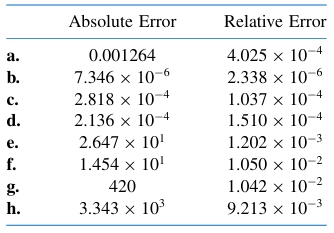
\includegraphics[width=8cm]{Mod1Sec1}
%%\end{center}
%\end{mysolution}
%
%
%%\begin{mysolution}
%%\begin{enumerate}[label=(\alph*)]
%%%\item  Absolute error is
%%%\[\left|\pi-\frac{22}{7}\right|=0.001264\]
%%%Relative error is
%%%\[\frac{\left|\pi-\frac{22}{7}\right|}{\pi}=4.025\times 10^{-4}\]
%%%\item Absolute error is
%%%\[\left|\pi-3.1416\right|=0.7346\times10^{-5}\]
%%%Relative error is
%%%\[\frac{\left|\pi-3.1416\right|}{\pi}=2.338\times 10^{-6}\]
%%%\item Absolute error is
%%%\[\left|e-2.718\right|=0.2818\times10^{-3}\]
%%%Relative error is
%%%\[\frac{\left|e-2.718\right|}{e}=1.037\times 10^{-4}\]
%%%\item Absolute error is
%%%\[\left|\sqrt{2}-1.414\right|=0.2136\times10^{-3}\]
%%%Relative error is
%%%\[\frac{\left|\sqrt{2}-1.414\right|}{\sqrt{2}}=1.510\times 10^{-4}\]
%%%\item Absolute error is
%%%\[\left|e^{10}-22000\right|=0.2647\times10^{2}\]
%%%Relative error is
%%%\[\frac{\left|e^{10}-22000\right|}{e^{10}}=1.202\times 10^{-3}\]
%%\item [(f)] Absolute error is
%%\[\left|10^{\pi}-1400\right|=0.1454\times10^{2}\]
%%Relative error is
%%\[\frac{\left|10^{\pi}-1400\right|}{10^{\pi}}=1.050\times 10^{-2}\]
%%\item [(g)] Absolute error is
%%\[\left|8!-39900\right|=0.42\times10^{3}\]
%%Relative error is
%%\[\frac{\left|8!-39900\right|}{8!}=1.047\times 10^{-2}\]
%%\item [(h)] Absolute error is
%%\[\left|9!-\sqrt{18 \pi}(9 / e)^{9}\right|=0.3343\times10^{4}\]
%%Relative error is
%%\[\frac{\left|9!-\sqrt{18 \pi}(9 / e)^{9}\right|}{9!}=9.213\times 10^{-3}\]
%%\end{enumerate}
%%\end{mysolution}
%
%
%
%
%
%
%
%
%%\activities
%%Read on Finite-digit arithmetic and nested arithmetic in pages \textcolor{red}{\bf page $22-28$} and then attempt the subsequent quiz
%%\begin{activity}[\cg Reading]
%%\begin{enumerate}
%%\item Burden, R. L., Faires, J. D., Burden, A. M. (2015). Numerical Analysis. Tenth Edition, Cengage Learning.\\
%%\end{enumerate}
%%\end{activity}
%%\mylink{https://www.youtube.com/watch?v=cK1WTCA6EpQ}
%
%
%
%
%
%%\begin{figure}[h]
%%\centering
%%\begin{tikzpicture}[line cap=round,line join=round,scale=0.7]
%%%\filldraw[color=gray] plot[domain=-1:2] (\x,{(\x)^2-2*(\x)});
%%%\filldraw[color=gray] plot[domain=-1:2] (\x,{4-(\x)^2});
%%%\filldraw[color=blue!20] plot[domain=1.57:4.7] (\x,{cos(\x r)});
%%%\draw[color=cyan,smooth,ultra thick] plot[domain=0.6:4.2] (\x,{2*cos(\x r)});
%%%\filldraw[color=gray] plot[domain=1.57:4.2] (\x,{-2*cos(\x r)}) -- (4.2,0);
%%\filldraw [color=gray!30!] (-4,3) -- (3,-4) -- ((4,-4) -- (4,3) -- (-4,3);
%%\draw[>=latex,->,color=black] (-4,0) -- (4,0)node[below] { $x$};
%%\draw[>=latex,->,color=black] (0,-4) -- (0,3)node[left] { $y$};
%%\draw[ultra thick,dashed,color=black] (1,-2) -- (1,3);
%%\draw[color=cyan,smooth,ultra thick] plot[domain=-4:3] (\x,{-(\x)-1});
%%%\draw[color=red,smooth,ultra thick] plot[domain=-2.5:2.5] (\x,{4-(\x)^2}) node [black, right] {\scriptsize $y=4-x^2$};
%%
%%%\filldraw [red] (2,0) circle (3pt);
%%
%%%\draw[ultra thick] (4.2,-1.05) -- (4.2,1.05);
%%%%\draw[dashed] (6.283,0) -- (6.283,1);
%%%%\foreach \y in {1,-1}
%%%%\draw[shift={(0,\y)},color=black] (2pt,0pt) -- (-2pt,0pt) node[left] {\footnotesize $\y$};
%%%%\draw[color=black] (0pt,-5pt) node[left] {\footnotesize $0$};
%%%
%%\draw[>=latex,->,color=black] (-1.5,3.2) -- (-2,1);
%%\draw(-1,0) node[below] {\scriptsize $-1$};
%%\draw(0,-1) node[left] {\scriptsize $-1$};
%%\draw(0,0) node[below left] {\scriptsize $0$};
%%\draw(1,2) node[right] {\scriptsize $x=1$};
%%\draw(-1.5,3.2) node [above] {\scriptsize $y=-x-1$};
%%%\draw(2.9,-0.5) node[] { $A_2$};
%%%\draw(1,0.8) node[above] { \scriptsize $y=\cos x$};
%%%\draw(2.9,2.2) node[above] { $y=|f(f)|$};
%%\end{tikzpicture}
%%\caption{\scriptsize Graph of $f(x,y)=\frac{\sqrt{x+y+1}}{x-1}$}
%%\label{firstexamplea}
%%\end{figure}
%
%
%%\begin{figure}%[h]
%%\centering
%%\begin{tikzpicture}[scale=1.5]
%%%\filldraw [color=gray!30!] (-2,-2) -- (-2,2) -- (2,2) -- (2,-2) -- (-2,-2);
%%    \draw[->] (-2,0) -- (2,0) node[right] {$x$};
%%    \draw[->] (0,-2) -- (0,2) node[above] {$y$};
%%    \draw[domain=0:1.5, smooth, variable=\x,blue] plot ({\x},{sqrt(\x)});
%%    \draw[domain=0:1.5, smooth, variable=\x,blue] plot ({\x},{-sqrt(\x)});
%%    \draw[dashed] (0,1.5) -- (1.5,1.5) node[right] {$y^2 = x$};
%%    \draw[dashed] (1.5,0) -- (1.5,1.5);
%%\end{tikzpicture}
%%\caption{\scriptsize Graph of $f(x,y)=x\ln(y^2-x)$}
%%\label{firstexampleb}
%%\end{figure}
%
%
%
%\section{Algorithms and Convergence}
%\begin{youtube}[]
%Watch the following video on  a discussion on algorithms and \\convergence as applied to numerical methods then attempt\\ the subsequent quiz.\\
%\mylink{https://www.youtube.com/watch?v=w7bJIRbgTvA\&t=51s}
%\end{youtube}
%\begin{myexercise}\label{Comprehensionquiz2}
%\begin{enumerate}[label=(\alph*)]
%\item Use three-digit chopping arithmetic to compute the sum $\sum_{i=1}^{10} 1 / i^{2}$ first by $\frac{1}{1}+\frac{1}{4}+\cdots+\frac{1}{100}$ and then by $\frac{1}{100}+\frac{1}{81}+\cdots+\frac{1}{1}$. Which method is more accurate, and why?
%\item Write an algorithm to sum the finite series $\sum^N_{i=1}x_i$ in reverse order.
%\end{enumerate}
%
%
%\begin{mysolution}
%\begin{enumerate}[label=(\alph*)]
%\item The forward order sum is
%\begin{center}
%\begin{tabular}{|l|l|l|}\hline
%$1/i^2$&Chopped Value&Running Total\\\hline
%$1$&$1.00$&$1.00$\\
%$0.25$&$0.250$&$1.00+0.250=1.25$\\
%$0.\bar{1}$&$0.111$&$1.25+0.111=1.36$\\
%$0.0625$&$0.062$&$1.36+0.062=1.42$\\
%$0.04$&$0.040$&$1.42+0.04=1.46$\\
%$0.02\bar{7}$&$0.027$&$1.46+0.027=1.48$\\
%$0.0204\ldots$&$0.020$&$1.48+0.020=1.50$\\
%$0.015625$&$0.015$&$1.50+0.015=1.51$\\
%$0.012345\ldots$&$0.012$&$1.51+0.012=1.52$\\
%$0.01$&$0.010$&$1.52+0.010=1.53$\\\hline
%\end{tabular}
%\end{center}
%%The backward order sum is
%%\begin{center}
%%\begin{tabular}{|l|l|l|}\hline
%%$1/i^2$&Chopped Value&Running Total\\\hline
%%$0.01$&$0.010$&$0.010$\\
%%$0.012345\ldots$&$0.012$&$0.010+0.012=0.022$\\
%%$0.015625$&$0.015$&$0.022+0.015=0.037$\\
%%$0.0204\ldots$&$0.020$&$0.037+0.020=0.057$\\
%%$0.02\bar{7}$&$0.027$&$0.057+0.027=0.084$\\
%%$0.04$&$0.040$&$0.084+0.04=0.124$\\
%%$0.0625$&$0.062$&$0.124+0.062=0.186$\\
%%$0.\bar{1}$&$0.111$&$0.186+0.111=0.297$\\
%%$0.25$&$0.250$&$0.297+0.250=0.547$\\
%%$1$&$1.00$&$0.5471.00=1.54$\\\hline
%%\end{tabular}
%%\end{center}
%%
%%
%%The exact value is
%%\[\sum_{i=1}^{10}(1/i^2)=1.54976773117\]
%
%\end{enumerate}
%\end{mysolution}
%
%%\newpage
%
%\begin{mysolution}
%\begin{enumerate}[label=(\alph*)]
%\item[]
%The backward order sum is
%\begin{center}
%\begin{tabular}{|l|l|l|}\hline
%$1/i^2$&Chopped Value&Running Total\\\hline
%$0.01$&$0.010$&$0.010$\\
%$0.012345\ldots$&$0.012$&$0.010+0.012=0.022$\\
%$0.015625$&$0.015$&$0.022+0.015=0.037$\\
%$0.0204\ldots$&$0.020$&$0.037+0.020=0.057$\\
%$0.02\bar{7}$&$0.027$&$0.057+0.027=0.084$\\
%$0.04$&$0.040$&$0.084+0.04=0.124$\\
%$0.0625$&$0.062$&$0.124+0.062=0.186$\\
%$0.\bar{1}$&$0.111$&$0.186+0.111=0.297$\\
%$0.25$&$0.250$&$0.297+0.250=0.547$\\
%$1$&$1.00$&$0.5471.00=1.54$\\\hline
%\end{tabular}
%\end{center}
%Thus
%\begin{center}
%\begin{tabular}{|l|l|l|}\hline
%Method&Sum&Absolute Error\\\hline
%Forward sum&$1.53$&$approx0.0198$\\
%Backward sum&$1.54$&$approx0.0098$\\\hline
%\end{tabular}
%\end{center}
%Hence the backward sum is more accurate. This is due to loss of significance in floating-point arithmetic.
%
%\begin{itemize}
%\item In forward order, large numbers (e.g., $1.00$) are added first.
%\item Later, small values (like $0.01$) may get lost due to limited precision; adding them to a large total may have no effect after chopping.
%\item In reverse order, we add small numbers first, so their contributions are preserved early in the summation.
%\item Later, adding large values doesn't suffer as much from chopping.
%\end{itemize}
%This is a classic example of numerical stability: summing from smallest to largest reduces round-off error.
%\item [(b)] Here is the algorithm
%
%\begin{boxB}
%Algorithm ReverseSum(x, N):\\
%Input: Array $x[1\ldots N]$ containing the series terms\\
%Output: Sum of the series $\sum_{i=1}^N x_i$, computed in reverse order\\
%\\
%Step 1 Set SUM=0\\
%Step 2 For $i=N, \ldots, 1$\\
%\hspace*{1cm} Set SUM=SUM+x\_i\\
%Step 3 Output (SUM)\\
%\hspace*{1cm} STOP
%\end{boxB}
%\end{enumerate}
%\end{mysolution}
%\end{myexercise}
%
%\section{Solution of Equations of One Variable}
%\videolesson
%\begin{selfvideo}[2]
%%LESSON 3: 
%This video covers bisection method for solving equation of one variable. Follow the discussion and attempt the quiz that follows.
%\end{selfvideo}
%%\begin{boxB}Question: Which are the determining factors for the temperature of a given location on the surface of the earth at a given time?\end{boxB}
%In this section we consider one of the most basic problems of numerical approximation, the {\bf root-finding problem}. This process involves finding a {\bf root}, or solution, of an equation of the form $f(x)=0$, for a given function $f$. A root of this equation is also called a {\bf zero} of the function $f$.
%
%\subsection*{Bisection Technique}
%Suppose $f$ is a continuous function defined on the interval $[a,b]$, with $f(a)$ and $f(b)$ of opposite sign. The Intermediate Value Theorem implies that a number $p$ exists in $(a,b)$ with $f(p) = 0$. Although the procedure will work when there is more than one root in the interval $(a, b)$, we assume for simplicity that the root in this interval is unique. The method calls for a repeated halving (or bisecting) of subintervals of $[a,b]$ and, at each step, locating the half containing $p$.
%
% To begin, set $a_1 = a$ and $b_1 = b$, and let $p_1$ be the midpoint of $[a,b]$; that is,
%\[p_1=a_1+\frac{b_1-a_1}{2}=\frac{a_1+b_1}{2}.\]
%\begin{itemize}
%\item If $f(p_1)=0$, then $p=p_1$, and we are done.
%\item If $f(p_1)\neq0$, then $f(p_1)$ has the same sign as either $f(a_1)$ or $f(b_1)$.
%\item If $f\left(p_{1}\right)$ and $f\left(a_{1}\right)$ have the same sign, $p\in(p_1,b_1)$. Set $a_{2}=p_{1}$ and $b_{2}=b_{1}$.
%\item If $f\left(p_{1}\right)$ and $f\left(a_{1}\right)$ have opposite signs, then $p\in(a_1,p_1)$. Set $a_{2}=a_{1}$ and $b_{2}=p_{1}$.
%\end{itemize}
%
%Then reapply the process to the interval $\left[a_{2}, b_{2}\right]$. (See Figure below)
%
%%%\begin{myalgorithm}
%%%\underline{To find a solution to $f(x) = 0$ given the continuous function $f$ on the interval $[a,b]$, where}\\
%%%\underline{ $f(a)$ and $f(b)$ have opposite signs:}\\
%%%%\begin{tabular}{ll}
%%%INPUT {\it endpoints $a, b$; tolerance TOL; maximum number of iterations $N_0$.}\\
%%%OUTPUT {\it approximate solution p or message of failure.}\\
%%%%\end{tabular}
%%%Step 1\hspace{1cm} Set $i=1$;\\
%%%\hspace{4cm} $FA=f(a)$\\
%%%Step 2\hspace{2cm} While $i\leq N_0$ do Steps $3-6$.\\
%%%~~~~~~Step 3\hspace{1cm} Set $p=a+(b-a)/2$; \hspace{1cm} ({\it Compute $p_i$})
%%%\hspace{5cm}
%%%\end{myalgorithm}
%%
%%\begin{tcolorbox}
%%\underline{\bf ALGORITHM $1$ To find a solution to $f(x) = 0$ given the continuous function $f$ on the}\\
%%\underline{\bf interval $[a,b]$, where $f(a)$ and $f(b)$ have opposite signs:}\\
%%INPUT {\it endpoints $a, b$; tolerance $TOL$; maximum number of iterations $N_0$.}\\
%%OUTPUT {\it approximate solution p or message of failure.}\\
%%Step 1 Set $i=1$;\\
%%\hspace*{2cm} $FA=f(a)$.\\
%%Step 2 While $i\leq N_0$ do Steps $3 - 6$.\\
%%\hspace*{1cm} Step 3 Set $p=a+(b-a)/2$; ({\it Compute$p_i$}.)\\
%%\hspace*{3cm}$FP=f(p)$.\\
%%\hspace*{1cm}  Step 4 If $FP=0$ or $(b-a)/2<TOL$ then \\
%%\hspace*{3cm} OUTPUT $(p)$; ({\it Procedure completed successfully}.)\\
%%\hspace*{3cm} STOP.\\
%%\hspace*{1cm} Step 5 Set $i=i+1$.\\
%%\hspace*{1cm} Step 6 If $FA\cdot FP>0$ then set $a=p$; ({\it Compute $a_i$, $b_i$.})\\
%%\hspace*{5cm} $FA=FP$\\
%%\hspace*{4cm} else set $b=p$. ({\it $FA$ is unchanged}.)\\
%%Step 7 OUTPUT (`Method failed after $N_0$ iterations, $N_0=', N_0$);\\
%%\hspace*{1cm} ({\it The procedure was unsuccessful}.)\\
%%\hspace*{1cm} STOP
%%\end{tcolorbox}
%
%\begin{figure}[h]
%\centering
%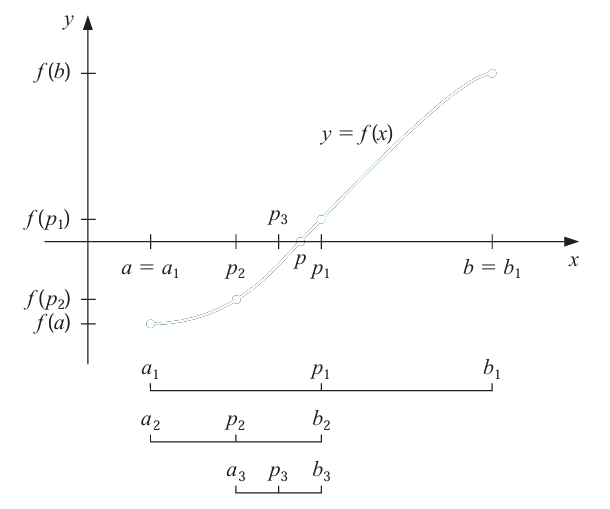
\includegraphics[ width=10cm]{Bisectionmethodpicture1.jpeg}
%\caption{\scriptsize }
%\label{}
%\end{figure}
%
%
%
%
%
%
%
%%[Bisection Method] An interval $\left[a_{n+1}, b_{n+1}\right]$ containing an approximation to a root of $f(x)=0$ is constructed from an interval $\left[a_{n}, b_{n}\right]$ containing the root by first letting
%%
%%$$
%%p_{n}=a_{n}+\frac{b_{n}-a_{n}}{2}
%%$$
%%
%%Then set
%%
%%$$
%%a_{n+1}=a_{n} \quad \text { and } \quad b_{n+1}=p_{n} \quad \text { if } \quad f\left(a_{n}\right) f\left(p_{n}\right)<0
%%$$
%%
%%and
%%
%%$$
%%a_{n+1}=p_{n} \quad \text { and } \quad b_{n+1}=b_{n} \quad \text { otherwise. }
%%$$
%%
%%There are three stopping criteria commonly incorporated in the Bisection method. First, the method stops if one of the midpoints happens to coincide with the root. It also stops when the length of the search interval is less than some prescribed tolerance we call $T O L$. The procedure also stops if the number of iterations exceeds a preset bound $N_{0}$.
%%
%%To start the Bisection method, an interval $[a, b]$ must be found with $f(a) \cdot f(b)<$ 0 . At each step, the length of the interval known to contain a zero of $f$ is reduced by a factor of 2 . Since the midpoint $p_{1}$ must be within $(b-a) / 2$ of the root $p$, and each succeeding iteration divides the interval under consideration by 2 , we have
%%
%%$$
%%\left|p_{n}-p\right| \leq \frac{b-a}{2^{n}}
%%$$
%%
%%As a consequence, it is easy to determine a bound for the number of iterations needed to ensure a given tolerance. If the root needs to be determined within the tolerance TOL, we need to determine the number of iterations, $n$, so that
%%
%%$$
%%\frac{b-a}{2^{n}}<T O L
%%$$
%%
%%Solving for $n$ in this inequality gives
%%
%%$$
%%\frac{b-a}{T O L}<2^{n}, \quad \text { which implies that } \quad \log _{2}\left(\frac{b-a}{\mathrm{TOL}}\right)<n .
%%$$
%%
%%Since the number of required iterations to guarantee a given accuracy depends on the length of the initial interval $[a, b]$, we want to choose this interval as small as possible. For example, if $f(x)=2 x^{3}-x^{2}+x-1$, we have both
%%
%%$$
%%f(-4) \cdot f(4)<0 \quad \text { and } \quad f(0) \cdot f(1)<0
%%$$
%%
%%so the Bisection method could be used on either $[-4,4]$ or $[0,1]$. Starting the Bisection method on $[0,1]$ instead of $[-4,4]$ reduces by 3 the number of iterations required to achieve a specified accuracy.
%%\end{itemize}
%\begin{example}
%Show that $f(x) = x^3 +4x^2 -10 = 0$ has a root in $[1,2]$, and use the Bisection method to determine an approximation to the root that is accurate to at least within $10^{-4}$.
%\end{example}
%
%\begin{mysolution}
%Because $f(1) =-5$ and $f(2) = 14$ the Intermediate Value Theorem ensures that this continuous function has a root in $[1,2]$. 
%
%For the first iteration of the Bisection method we use the fact that at the midpoint of $[1, 2]$ we have $f(1.5) = 2.375 > 0$. This indicates that we should select the interval $[1,1.5]$ for our second iteration. Then we find that $f(1.25) =-1.796875$ so our new interval becomes $[1.25,1.5]$, whose midpoint is $1.375$. Continuing in this manner gives the values in Table \ref{}. After $13$ iterations, $p_{13} = 1.365112305$ approximates the root $p$ with an error
%\[|p-p_{13}|<|b_{14}-a_{14}|=|1.365234375-1.365112305|=0.000122070.\]
%Since $|a_{14}|<|p|$, we have
%\[\frac{|p-p_{13}|}{|p|}<\frac{|b_{14}-a_{14}|}{|a_{14}|}\leq9.0\times10^{-5},\]
%so the approximation is correct to atleast within $10^{-4}$. The correct value of $p$ to nine decimal  places is $p=1.365230013$. Note that $p_9$ is closer to $p$ than is the final approximation $p_{13}$.
%
%\begin{center}
%\centering
%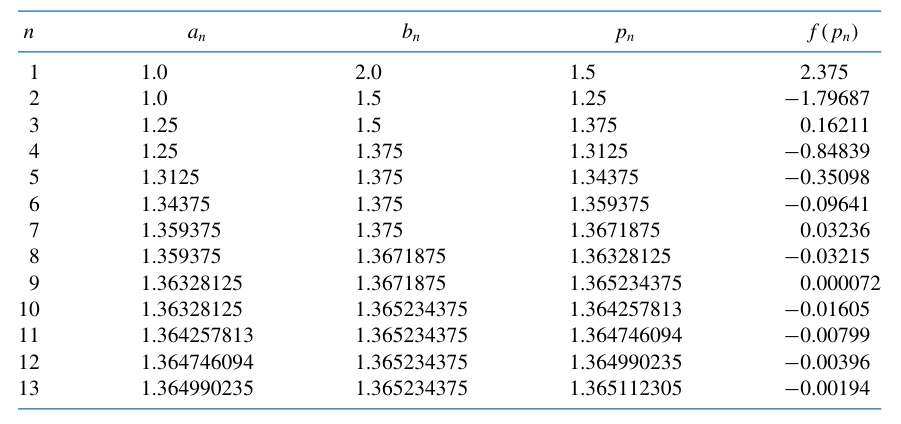
\includegraphics[ width=13cm]{Bisectionmethodexampletable.jpeg}
%%\caption{\scriptsize }
%%\label{}
%\end{center}
%\end{mysolution}
%
%\begin{theorem}
%Suppose that $f\in C[a, b]$ and $f(a)\cdot f(b)<0$. The Bisection method generates a sequence $\left\{p_n\right\}_{n=1}^{\infty}$ approximating a zero $p$ of $f$ with
%\[|p_n-p|\leq\frac{b-a}{2^n},\quad\mbox{when}\quad n\geq1.\]
%\end{theorem}
%
%\begin{example}
%Determine the number of iterations necessary to solve $f(x) = x^3 + 4x^2 - 10 = 0$ with accuracy $10^{-3}$  using $a_1 = 1$ and $b_1 = 2$.
%\end{example}
%
%\begin{mysolution}
%We we will use logarithms to find an integer $N$ that satisfies
%\[|p_N-p|\leq2^{-N}(b-a)=2^{-N}<10^{-3}.\]
%Logarithms to any base would suffice, but we will use base$-10$ logarithms because the tolerance is given as a power of $10$. Since $2^{-N}<10^{-3}$ implies that $\log_{10}2^{-N}<\log_{10}10^{-3} =-3$, we have
%\[-N\log_{10}2<-3\quad\mbox{and}\quad N>\frac{3}{\log_{10}2}\approx9.96.\]
%Hence, ten iterations will ensure an approximation accurate to within $10^{-3}$.
%
%Table \ref{} shows that the value of $p_9 = 1.365234375$ is accurate to within $10^{-4}$. Again, it is important to keep in mind that the error analysis gives only a bound for the number of iterations. In many cases this bound is much larger than the actual number required.
%\end{mysolution}
%
%\begin{myexercise}\label{Comprehensionquiz2}
%\begin{enumerate}[label=\arabic*.]
%\item Use the Bisection method to find $p_{3}$ for $f(x)=\sqrt{x}-\cos x$ on $[0,1]$. 
%\item Use the Bisection method to find solutions accurate to within $10^{-2}$ for $x^{3}-$ $7 x^{2}+14 x-6=0$ on each interval.
%\begin{multicols}{3}
%\begin{enumerate}[label=(\alph*)]
%\item $[0,1]$
%\item $[1,3.2]$
%\item $[3.2,4]$
%\end{enumerate}
%\end{multicols}
%\end{enumerate}
%
%\begin{mysolution}
%\begin{enumerate}[label=\arabic*.]
%\item Here $f(0)=-1<0$ and $f(1)=0.45969769413>0$. The sequence of approximate solutions are tabulated below
%
%\begin{center}
%\begin{tabular}{lllll}\hline
%$n$&$a_n$&$b_n$&$p_n$&$f(p_n)$\\
%$1$&$0$&$1$&$0.5$&$-0.1704757807$\\
%$2$&$0.5$&$1$&$0.75$&$0.13433653491$\\
%$3$&$0.5$&$0.75$&$0.625$&$-0.02039370446$\\\hline
%\end{tabular}
%\end{center}
%$p_3=0.625$
%
%\item 
%\begin{enumerate}[label=(\alph*)]
%\item Here $a=0$ and $b=1$ so that $2^{-n}<10^{-2}$. Applying natural logarithm to both sides of the inequality yields $log_{10}2^{-n}<log_{10}10^{-2}$. Solving for $n$ yields 
%\[n>\frac{2}{log_{10}2}=6.643\ldots\]
%
%Thus $n=7$. Here $f(0)=-6<0$ and $f(1)=2>0$. The sequence of approximate solutions are tabulated below
%\end{enumerate}
%\end{enumerate}
%\end{mysolution}
%%
%\begin{mysolution}
%\begin{enumerate}
%\item[]
%
%\begin{center}
%\begin{tabular}{lllll}\hline
%$n$&$a_n$&$b_n$&$p_n$&$f(p_n)$\\
%$1$&$0$&$1$&$0.5$&$-0.625$\\
%$2$&$0.5$&$1$&$0.75$&$0.984375$\\
%$3$&$0.5$&$0.75$&$0.625$&$0.259765625$\\
%$4$&$0.5$&$0.625$&$0.5625$&$-0.16186523438$\\
%$5$&$0.5625$&$0.625$&$0.59375$&$0.29712163086$\\
%$6$&$0.5625$&$0.59375$&$0.578125$&$-0.05262374878$\\\hline
%\end{tabular}
%\end{center}
%
%\vspace{3mm}
%$p_7=\frac{0.578125+0.59375}{2}=0.5859$ 
%
%\begin{enumerate}
%\item[(b)] Here $a=1$ and $b=3.2$ so that $2^{-n}\cdot2.2<10^{-2}$. Applying natural logarithm to both sides of the inequality yields $log_{10}2^{-n}<log_{10}10^{-2}-log_{10}2.2$. Solving for $n$ yields 
%\[n>\frac{2+log_{10}2.2}{log_{10}2}=7.781\]
%Thus $n=8$. Here $f(1)=2>0$ and $f(3.2)=-0.112<0$. The sequence of approximate solutions are tabulated below
%\begin{center}
%\begin{tabular}{lllll}\hline
%$n$&$a_n$&$b_n$&$p_n$&$f(p_n)$\\
%$1$&$1$&$3.2$&$2.1$&$1.791$\\
%$2$&$2.1$&$3.2$&$2.65$&$0.552125$\\
%$3$&$2.65$&$3.2$&$2.925$&$0.085828125$\\
%$4$&$2.925$&$3.2$&$3.0625$&$-0.5444335938$\\
%$5$&$2.925$&$3.0625$&$2.99375$&$0.00632788086$\\
%$6$&$2.99375$&$3.0625$&$3.028125$&$-0.02652072144$\\
%$7$&$2.99375$&$3.028125$&$3.0109375$&$-0.01069693375$\\\hline
%\end{tabular}
%\end{center}
%%\end{enumerate}
%%\end{enumerate}
%%\end{mysolution}
%%
%%\begin{mysolution}
%%\begin{enumerate}
%%\item[]
%%\begin{enumerate}
%%\item[]
%$p_8=\frac{2.99375+3.028125}{2}=3.002$
%
%\vspace{5mm}
%
%
%\item [(c)] Here $a=3.2$ and $b=4$ so that $2^{-n}\cdot0.8<10^{-2}$. Applying natural logarithm to both sides of the inequality yields $log_{10}2^{-n}<log_{10}10^{-2}-log_{10}0.8$. Solving for $n$ yields 
%\[n>\frac{2+log_{10}0.8}{log_{10}2}=6.32192\ldots\]
%Thus $n=7$. Here $f(3.2)=-0.112<0$ and $f(4)=2>0$. The sequence of approximate solutions are tabulated below
%\begin{center}
%\begin{tabular}{lllll}\hline
%$n$&$a_n$&$b_n$&$p_n$&$f(p_n)$\\
%$1$&$3.2$&$4$&$3.6$&$0.336$\\
%$2$&$3.2$&$3.6$&$3.4$&$-0.016$\\
%$3$&$3.4$&$3.6$&$3.5$&$0.125$\\
%$4$&$3.4$&$3.5$&$3.45$&$0.046125$\\
%$5$&$3.4$&$3.45$&$3.425$&$0.013015625$\\
%$6$&$3.4$&$3.425$&$3.4125$&$-0.00199804688$\\\hline
%\end{tabular}
%\end{center}
%
%\vspace{3mm}
%$p_7=\frac{3.4125+3.425}{2}=3.419$
%\end{enumerate}
%\end{enumerate}
%\end{mysolution}
%\end{myexercise}
% 
%
%\section{Fixed Point Iteration and Newton's Method}
%\activities
%Read on Newton's Method and its extensions in pages in the link below and then attempt the subsequent quiz
%\begin{activity}[\cg Reading]
%%\begin{enumerate}
%%\textcolor{red}{\bf page $934-946$}
%%\item Ryan T. White and Archana Tikayat Ray, (2021), {\it Practical Discrete Mathematics: Discover math principles that fuel algorithms for computer science and machine learning with Python}, Packt Publishing,  ISBN-13 ‏ : ‎ 978-1838983147 \\
%%\textcolor{red}{\bf pages $23-30$}
%%\item S. Lipschutz and M. Lipson, (2021), {\it Schaum’s Outline of Discrete Mathematics}, Fourth Edition (Schaum’s Outlines) 4th Edition, McGraw Hill, ISBN-13: 978-1264258802\\
%%\textcolor{red}{\bf pages $70-76$}
%%\end{enumerate}
%\end{activity}
%\mylink{https://pythonnumericalmethods.studentorg.berkeley.edu/notebooks/chapter19.04-Newton-Raphson-Method.html}\\
%\begin{youtube}[]
%Watch the following video on  a discussion on Fixed-Point Iteration then attempt the subsequent quiz.\\
%\mylink{https://www.youtube.com/watch?v=I-B9MGK3gwU}
%\end{youtube}
%
%\begin{myexercise}\label{Comprehensionquiz2}
%\begin{enumerate}[label=\arabic*.]
%\item Use algebraic manipulation to show that each of the following functions has a fixed point at $p$ precisely
% when $f(p) = 0$, where $f(x) = x^4 +2x^2-x-3$.
%\begin{multicols}{2}
%\begin{enumerate}[label=(\alph*)]
%\item $g_1(x)=(3+x-2x^2)^{1/4}$\\[5mm]
%\item $g_2(x)=\left(\frac{x+3-x^4}{2}\right)^{1/2}$
%\item $g_3(x)=\left(\frac{x+3}{x^2+2}\right)^{1/2}$\\[4mm]
%\item $g_4(x)=\frac{3x^4+2x^2+3}{4x^4+4x-1}$
%\end{enumerate}
%\end{multicols}
%\item Let $f(x)=x^2−6$ and $p_0=1$. Use Newton’s method to find $p_2$.
%\begin{mysolution}
%\begin{enumerate}[label=(\alph*)]
%\item For the value of $x$ under consideration we have
%%\begin{multicols}{2}
%\begin{enumerate}[label=\arabic*.]
%\item $x =(3+x-2x^2)^{1/4}\quad\Leftrightarrow\quad x^4 = 3+x-2x^2\quad\Leftrightarrow\quad f(x) = 0$\\
%\item $x =\left(\frac{x+3-x^4}{2}\right)^{1/2}\quad\Leftrightarrow\quad 2x^2 = x+3-x^4\quad\Leftrightarrow\quad f(x) = 0$\\
%\item $x =\left(\frac{x+3}{x^2+2}\right)^{1/2}\quad\Leftrightarrow\quad x^2(x^2+2)= x+3\quad\Leftrightarrow\quad f(x) = 0$\\
%\item $x =\frac{3x^4+2x^2+3}{4x^3+4x-1}\quad\Leftrightarrow\quad 4x^4+4x^2-x= 3x^4+2x^2+3\quad\Leftrightarrow\quad f(x) = 0$
%\end{enumerate}
%%\end{multicols}
%\item $p_2=2.60714$
%\end{enumerate}
%\end{mysolution}
%\end{enumerate}
%\end{myexercise}
%
%
%
%
%
%
%%%%%%%%%%%%%%%%%%%%%%%%%%%%%%%%%%%%%%%%%%%%%%%%%%%%%%%%%%%%%%%%%%%%%%%%%%%%%%%%%%%%%%%%%%%%%%%%%%%%%%%%%%%%%%%%%%%%%%%%%%%%%%%%%%%%%%%%%%%%%%%
%
%
%
%%\bibliographystyle{unsrt} \bibliography{bibliography}
%
%%\activities
%%The following reading is necessary for your constructive engagement in the group discussion.
%%\begin{activity}[\cg Reading]
%%\begin{enumerate}
%%\item Burden, R. L., Faires, J. D., Burden, A. M. (2015). Numerical Analysis. Tenth Edition, Cengage Learning.\\
%%%\textcolor{red}{\bf page $934-946$}
%%%\item Ryan T. White and Archana Tikayat Ray, (2021), {\it Practical Discrete Mathematics: Discover math principles that fuel algorithms for computer science and machine learning with Python}, Packt Publishing,  ISBN-13 ‏ : ‎ 978-1838983147 \\
%%%\textcolor{red}{\bf pages $23-30$}
%%%\item S. Lipschutz and M. Lipson, (2021), {\it Schaum’s Outline of Discrete Mathematics}, Fourth Edition (Schaum’s Outlines) 4th Edition, McGraw Hill, ISBN-13: 978-1264258802\\
%%%\textcolor{red}{\bf pages $70-76$}
%%\end{enumerate}
%%\end{activity}
%
%%\discussion
%%Discuss how you would solve questions 71-75 in Exercise 14.1 of indicated reference.
%
%%\begin{enumerate}
%%\item Render the implication in English language.
%%\item\label{Discusion1} Determine the converse, contrapositive and inverse of the implication $u\rightarrow v$  in symbolic notation in terms of the component propositions
%%\item Express each of the implications obtained in \ref{Discusion1} English language
%%\end{enumerate}
%
%
%%Let $p$, $q$, $r$, and $s$ be the following propositions
%%\[\begin{split}
%%p:&~ \mbox{Grizzly bears have been seen in the area.}\\
%%q:&~  \mbox{Hiking is safe on the trail.}\\
%%r:&~  \mbox{Berries are ripe along the trail.}\\
%%s:&~  \mbox{You drive over 65 miles per hour.}
%%\end{split}\]
%%
%%Consider the following implication $u\rightarrow v$ where
%%\[u:\neg(p\lor q)\quad\mbox{ and }\quad v:r\lor\neg s.\]
%
%%\begin{enumerate}
%%\item Render the implication in English language.
%%\item\label{Discusion1} Determine the converse, contrapositive and inverse of the implication $u\rightarrow v$  in symbolic notation in terms of the component propositions
%%\item Express each of the implications obtained in \ref{Discusion1} English language
%%\end{enumerate}
%%Thank you and keep safe!
%
%\begin{posttest}[\textcolor{red}{End of Module One Quiz}]
%\item Suppose $p^*$ must approximate $p$ with relative error at most $10^{-3}$. Find the largest interval in which $p^*$ must lie for each value of $p$.
%\begin{multicols}{4}
%\begin{enumerate}[label=(\alph*)]
%\item $150$
%\item $900$
%\item $1500$
%\item $90$
%\end{enumerate}
%\end{multicols}
%\begin{mysolution}
%\begin{enumerate}[label=(\alph*)]
%\item[]
%\[\frac{|p^*-p|}{|p|}\leq10^{-3}\quad\Longleftrightarrow\quad p\left(1-10^{-3}\right)\leq p^*\leq p\left(1+10^{-3}\right)\]
%\item Here $p=150$ so that $p\left(1-10^{-3}\right)=150\left(1-10^{-3}\right)=149.85$ and $p\left(1+10^{-3}\right)=150\left(1+10^{-3}\right)=150.15$. Hence the required interval is $(149.85,150.15)$
%\item Here $p=900$ so that $p\left(1-10^{-3}\right)=900\left(1-10^{-3}\right)=899.1$ and $p\left(1+10^{-3}\right)=900\left(1+10^{-3}\right)=900.9$. Hence the required interval is $(899.1,900.9)$
%\item Here $p=1500$ so that $p\left(1-10^{-3}\right)=1500\left(1-10^{-3}\right)=1498.5$ and $p\left(1+10^{-3}\right)=1500\left(1+10^{-3}\right)=1501.5$. Hence the required interval is $(1498.5,1501.5)$
%\item Here $p=90$ so that $p\left(1-10^{-3}\right)=90\left(1-10^{-3}\right)=89.91$ and $p\left(1+10^{-3}\right)=90\left(1+10^{-3}\right)=90.09$. Hence the required interval is $(89.91,90.09)$
%\end{enumerate}
%
%\end{mysolution}
%\item The Maclaurin series for the arctangent function converges for $-1<x \leq 1$ and is given by
%
%$$
%\arctan x=\lim _{n \rightarrow \infty} P_{n}(x)=\lim _{n \rightarrow \infty} \sum_{i=1}^{n}(-1)^{i+1} \frac{x^{2 i-1}}{(2 i-1)}
%$$
%
%\begin{enumerate}[label=(\alph*)]
%\item Use the fact that $\tan \pi / 4=1$ to determine the number of terms of the series that need to be summed to ensure that $\left|4 P_{n}(1)-\pi\right|<10^{-3}$.
%\item The C programming language requires the value of $\pi$ to be within $10^{-10}$. How many terms of the series would we need to sum to obtain this degree of accuracy?
%\end{enumerate}
%\begin{mysolution}
%From the equation
%\[\arctan x=\lim _{n \rightarrow \infty} P_{n}(x)=\lim _{n \rightarrow \infty} \sum_{i=1}^{n}(-1)^{i+1} \frac{x^{2 i-1}}{(2 i-1)}\]
%it follows that 
%\[\frac{\pi}{4}=\arctan 1=\sum_{i=1}^{\infty}\frac{(-1)^{i+1}}{(2 i-1)}\]
%Therefore
%\[\frac{\pi}{4}\approx\sum_{i=1}^{n}\frac{(-1)^{i+1}}{(2 i-1)}\]
%This is an alternating series with terms which are decreasing in magnitude. Thus by the Alternating Series Remainder Theorem, the error $|4P_n(1)-\pi|$ is less than or equal to the absolute value of the first omitted term which is
%\[\left|\frac{(-1)^{(n+1)-1}\cdot 4}{2(n+1)-1}\right|=\frac{4}{2n+1}\]
%\begin{enumerate}[label=(\alph*)]
%\item Here we look for $n$ such that
%\[\frac{4}{2n+1}<10^{-3}\quad\Longleftrightarrow\quad n>\frac{4-10^{-3}}{2\times10^{-3}}=1999.5\]
%Thus the least such integer $n$ is $2000$ which is the required number of terms.
%\item Here we look for $n$ such that
%\[\frac{4}{2n+1}<10^{-10}\quad\Longleftrightarrow\quad n>\frac{4-10^{-10}}{2\times10^{-10}}=19,999,999,999.5\]
%Thus the least such integer $n$ is $20,000,000,000$ which is the required number of terms.
%\end{enumerate}
%\end{mysolution}
%\item Use the Bisection method to find solutions accurate to within $10^{-3}$ for the following problems.
%\begin{enumerate}[label=(\alph*)]
%\item $x-2^{-x}=0$ for $0\leq x\leq1$
%\item $e^x-x^2+3x-2=0$ for $0\leq x\leq1$
%%\item $2x\cos(2x)-(x+1)^2=0$ for $-3\leq x\leq-2$ and $-1\leq x\leq0$.
%%\item $x\cos x-2x^2+3x-1=0$ for $0.2\leq x\leq0.3$ and $1.2\leq x\leq1.3$
%\end{enumerate}
%\begin{mysolution}
%\begin{enumerate}[label=(\alph*)]
%\item Here $a=0$ and $b=1$. So in the inequality $2^{-n}(b-a)<10^{-3}$ becomes $2^{-n}(1-0)<10^{-3}$. Solving for $n$ obtain $n>\frac{3}{log_{10}2}=9.96578428466\ldots$ so that $n=10$.
%
%Now $f(0)=-1<0$ and $f(1)=0.5>0$. The sequence of approximate solutions are tabulated below
%\begin{center}
%\begin{tabular}{lllll}\hline
%$n$&$a_n$&$b_n$&$p_n$&$f(p_n)$\\
%$1$&$0$&$1$&$0.5$&$-0.20710678119$\\
%$2$&$0.5$&$1$&$0.75$&$0.1553964425$\\
%$3$&$0.5$&$0.75$&$0.625$&$-0.02341977733$\\
%$4$&$0.625$&$0.75$&$0.6875$&$0.06657109396$\\
%$5$&$0.625$&$0.6875$&$0.65625$&$0.0217245214$\\
%$6$&$0.625$&$0.65625$&$0.640625$&$-0.00081000804$\\
%$7$&$0.640625$&$0.65625$&$0.6484375$&$0.0074666108$\\
%$8$&$0.640625$&$0.6484375$&$0.64453125$&$0.00483064625$\\
%$9$&$0.640625$&$0.64453125$&$0.642578125$&$0.00201090611$\\\hline
%\end{tabular}
%\end{center}
%
%\vspace{3mm}
%$p_{10}=\frac{0.640625+0.64453125}{2}=0.642578125$
%\item Here $a=0$ and $b-1$. So in the inequality $2^{-n}(b-a)<10^{-3}$ becomes $2^{-n}(1-0)<10^{-3}$. Solving for $n$ obtain $n>\frac{3}{log_{10}2}=9.96578428466\ldots$ so that $n=10$.
%
%Now $f(0)=-1<0$ and $f(1)=2.71828\ldots>0$. The sequence of approximate solutions are tabulated below
%\begin{center}
%\begin{tabular}{lllll}\hline
%$n$&$a_n$&$b_n$&$p_n$&$f(p_n)$\\
%$1$&$0$&$1$&$0.5$&$0.8987212707$\\
%$2$&$0$&$0.5$&$0.25$&$-0.02847458331$\\
%$3$&$0.25$&$0.5$&$0.375$&$0.43936641462$\\
%$4$&$0.25$&$0.375$&$0.3125$&$0.20668169117$\\
%$5$&$0.25$&$0.3125$&$0.28125$&$0.08943319623$\\
%$6$&$0.25$&$0.28125$&$0.265625$&$0.03056423414$\\
%$7$&$0.25$&$0.265625$&$0.2578125$&$0.00106636769$\\
%$8$&$0.25$&$0.2578125$&$0.25390625$&$-0.01369868371$\\
%$9$&$0.25390625$&$0.2578125$&$0.255859375$&$-0.00631480679$\\
%\hline
%\end{tabular}
%\end{center}
%
%
%\vspace{3mm}
%$p_{10}=\frac{0.255859375+0.2578125}{2}=0.2568359375$
%%\item For the interval $[-3,-2]$, we have $p_{17} =-2.191307$, and for the interval $[-1,0]$, we have $p_{17}=-0.798164$.
%%\item For the interval $[0.2,0.3]$, we have $p_{14} =0.297528$, and for the interval $[1.2,1.3]$, we have $p_{14}=1.256622$.
%\end{enumerate}
%\end{mysolution}
%\item Let $f(x) = (x+2)(x+1)x(x-1)^3(x-2)$. To which zero of $f$ does the Bisection method converge when applied on the following intervals?
%\begin{multicols}{4}
% \begin{enumerate}[label=(\alph*)]
%\item $[-3,2.5]$
%\item $[-2.5,3]$
% \item $[-1.75,1.5]$
%\item $[-1.5,1.75]$
%\end{enumerate}
%\end{multicols}
%\begin{mysolution}
% \begin{enumerate}[label=(\alph*)]
%\item Here $a=-3$ and $b=2.5$ with $f(-3)<0$ and $f(2.5)>0$. We determine the zero of convergence in the table below where $m_n=(a_n+b_n)/2$
%
%\begin{center}
%\begin{tabular}{lllclc}\hline
%$n$&$a_n$&$b_n$&Zeros here&$m_n$&Sign of $f(m_n)$\\\hline
%$1$&$-3$&$2.5$&$-2, -1, 0, 1, 2$&$-0.25$&$-$\\
%$2$&$-0.25$&$2.5$&$0, 1, 2$&$1.125$&$-$\\\hline
%\end{tabular}
%\end{center} 
%
%The subsequent interval is $[1.125,2.5]$ and the only zero there is $2$.
%\item Here $a=-2.5$ and $b=3$ with $f(-2.5)<0$ and $f(3)>0$. We determine the zero of convergence in the table below where $m_n=(a_n+b_n)/2$
%
%\begin{center}
%\begin{tabular}{lllclc}\hline
%$n$&$a_n$&$b_n$&Zeros here&$m_n$&Sign of $f(m_n)$\\\hline
%$1$&$-2.5$&$3$&$-2, -1, 0, 1, 2$&$0.25$&$+$\\
%$2$&$-2.5$&$0.25$&$-2, -1, 0$&$-1.125$&$+$\\\hline
%\end{tabular}
%\end{center} 
%
%The subsequent interval is $[-2.5,-1.125]$ and the only zero there is $-2$.
% \item Here $a=-1.75$ and $b=1.5$ with $f(-1.75)>0$ and $f(1.5)<0$. We determine the zero of convergence in the table below where $m_n=(a_n+b_n)/2$
%
%\begin{center}
%\begin{tabular}{lllclc}\hline
%$n$&$a_n$&$b_n$&Zeros here&$m_n$&Sign of $f(m_n)$\\\hline
%$1$&$-1.75$&$1.5$&$-1, 0, 1$&$-0.125$&$-$\\\hline
%\end{tabular}
%\end{center} 
%
%The subsequent interval is $[-1.75,-0.125]$ and the only zero there is $-1$.
%\item  Here $a=-1.5$ and $b=1.75$ with $f(-1.5)>0$ and $f(1.75)<0$. We determine the zero of convergence in the table below where $m_n=(a_n+b_n)/2$
%
%\begin{center}
%\begin{tabular}{lllclc}\hline
%$n$&$a_n$&$b_n$&Zeros here&$m_n$&Sign of $f(m_n)$\\\hline
%$1$&$-1.5$&$1.75$&$-1, 0, 1$&$0.125$&$-$\\\hline
%\end{tabular}
%\end{center} 
%
%The subsequent interval is $[0.125,1.75]$ and the only zero there is $1$.
%\end{enumerate}
%\end{mysolution}
%
%\item The following four methods are proposed to compute $21^{1/3}$. Rank them in order, based on their
% apparent speed of convergence, assuming $p_0=1$.
%\begin{multicols}{2}
% \begin{enumerate}[label=(\alph*)]
%\item $p_n=\frac{20p_{n-1}+21/p_{n-1}^2}{21}$
%\item $p_n=p_{n-1}-\frac{p_{n-1}^3-21}{3p_{n-1}^2}$
%\item $p_n=p_{n-1}-\frac{p_{n-1}^4-21p_{n-1}}{p_{n-1}^2-21}$
%\item $p_n=\left(\frac{21}{p_{n-1}}\right)^{1/2}$
%\end{enumerate}
%\end{multicols}
%
%\begin{mysolution}
%The order in descending speed of convergence is (b), (d), (a). The sequence in (c) does not converge.
%\end{mysolution}
%%\item Find the domain and range of the function $f(x,y)=\sqrt{36-9x^2-9y^2}$.
%%\item Find the domain of the function $h(x,y,t)=(3t-6)\sqrt{y-4x^2+4}$
%%\item Find and graph the level curve of the function $g(x,y)=x^2+y^2-6x+2y$ corresponding to $k=15$.
%%\item Determine the equation of the vertical trace of the function $g(x,y)=-x^2-y^2+2x+4y-1$ corresponding to $y=3$, and describe the graph.
%%% Assume the population of a city is tripling every 5 years. If its current population is 10000, what will be the approximate population 2 years from now?\\
%%%Solution: Current population $P(0)=10000$ after 5 years $P(5)=30000$\\
%%%The gradient function $m$  gives the rate of change of population $P^'$;\\[0.1in]\\
%%%$P^'=\frac{P(5)-P(0)}{5-0}= \frac{30000-10000}{5-0}= 4000$\\[0.1in]\\
%%%By definition $P(2)=P(5)-m(5-2)$\\[0.1in]\\
%%%$P(2)=30000-4000(3)= 18000$, hence population after 2 years is 18000
%\end{posttest}
%
%
%\takehome
%
%%\comy{Good evening, you are now at the last part of this module. Your  task is to do a self-reflection on your learning experience.}
%\begin{itemize}
%\item In your own words what are some of your engagements/tasks in daily life where you can apply concepts of functions of several variables.
%\end{itemize}
%%
\begin{center}
    {\Large \textbf{FUNCTIONS OF SEVERAL VARIABLES}}\\[2mm]
(DEFINITION, DOMAIN, RANGE, GRAPHS AND LEVEL CURVES) \\[4mm]

\mycenterbox{5 minute review}%\\[4mm]
Recap the definition of a function of several variables, and the meaning of domain, range, graph and level curves of functions of several variables.
\end{center}
\mycenterbox{Warm-up.}%\\[4mm]
\problemAnswer{
Match the function with its graph (labeled I–VI).Give reasons for your choices
\begin{multicols}{3}
\begin{enumerate}[label=(\alph*)]
\item $f(x,y)=|x|+|y|$\\[4mm]
\item $f(x,y)=|xy|$
\item $f(x,y)=\frac{1}{1+x^2+y^2}$\\2mm]
\item $f(x,y)=(x^2-y^2)^2$
\item $f(x,y)=(x-y)^2$\\[4mm]
\item $f(x,y)=\sin(|x|+|y|)$
\end{enumerate}
\end{multicols}

\begin{center}
%\centering
\includegraphics[width=10cm]{MCTutorial1Q1.JPEG}
\end{center}
%\tcbox[tcbox raise base]{Warm-up}
 
%\begin{flushright}
%\begin{tikzpicture}
%    % A body
%
%
%    % Non-rectangle shapes must be drawn as polygone
%    \begin{scope}[shift={(3,0)}]
%        \draw  (0,0.5) -- (0,4) -- (.5,4) -- (.5,4.5) -- (1.,4.5) -- (4.,4.5) --(4.,4)-- (4.5,4) --(4.5,0.5) --(4.0,0.5)--(4.0,0.0)-- (.5,0) --(0.5,0.5) -- cycle;
%        % Draw symmetry lines
%        \draw [symmetry] (.5, 0.5) -- (.5,4.0);
%        \draw [symmetry] (4, 0.5) -- (4,4.0);
%        \draw [symmetry] (.5,4.0) -- (4,4.0);
%         \draw [symmetry] (.5, 0.5) -- (4, 0.5);
%        % Dimensions
%        \draw (4.5,0) -- ++(0.5,0) coordinate (D1) -- +(5pt,0);
%        \draw (4.5,4.5) -- ++(0.5,0) coordinate (D2) -- +(5pt,0);
%        \draw [dimen] (D1) -- (D2) node {6cm};
%       
%        
%        \draw (0.0,5) -- ++(0,0.5) coordinate (D1) -- +(0,+5pt);
%        \draw (0.5,5) -- ++(0,0.5) coordinate (D2) -- +(0,+5pt);
%        \draw [dimen,-] (D1) -- (D2) node [above=5pt] {$x$ cm};
%        \draw [dimen,<-] (D1) -- ++(-5pt,0);
%        \draw [dimen,<-] (D2) -- ++(+5pt,0);
%    \end{scope}
%\end{tikzpicture}
%\end{flushright}

}


\mycenterbox{Problems.}%

%\begin{center}
%\tcbox[tcbox raise base]{ Problems. Choose from the below}
%\end{center}
\problem{Exploring functions}%
\begin{enumerate}[(a)]
\item Are the following functions even, odd, or neither? What can you say
about their range?
\begin{multicols}{4}
 \begin{enumerate}[(i)]
\item $\displaystyle \frac{3x}{x^2+2}$
\item $\displaystyle \cos x+3$
\item $\displaystyle \frac{2x^3}{\cos x+3}$
\item $\displaystyle \frac{3x^4+2x^2}{\sin x+4}$
\end{enumerate}
\end{multicols}
\item Consider the functions $\sin^n x$ and $\cos^n x$, where $n$ is a positive integer.
Which are odd, which are even, and what are their periodicities?
\item What is the periodicity of $f(x) = 2 \cos x+\sin 2x$? Is it even/odd/neither?

\end{enumerate}

\problem{Cubic functions} 
Show that $x-1$ is a factor of the cubic function%
$$P(x)=x^3-2x^2-5x+6,$$
and  find the quadratic factor $Q(x)$ such that $P(x) = (x -1)Q(x)$. Factorise
$Q(x)$ and hence sketch $P(x).$

%\newpage
\problem{Sigmoid functions*.}%
For positive integers $n$, consider the family of functions
$$\displaystyle f_n= \frac{x^n}{2^n+x^n}.$$
\begin{enumerate}[(a)]
\item What are appropriate domains and ranges for $f_n(x)$? Do they depend on $n$?

\item Is $f_n(x)$ even, odd, or neither? Does this depend on $n$?

\item Show that for $x\geq 0$, $f_n(x)$ are strictly increasing functions and that
$0\leq f_n(x) < 1.$
\item What is the value of $f_n(2)$? Does it depend on $n$?

\item By considering the values of $f_n(1.9)$ and $f_n(2.1)$ for $n = 2, 4, 8, 16, 32$ and
$64$, show that the graph of $f_n(x)$ for $x\ge 0$ is an increasing sigmoid (that
is, $S$-shaped) function that approaches a step function as $n\rightarrow \infty$.
\end{enumerate}

\mycenterbox{Selected answers and hints}%

For the warm-up, $V(x)=4x(3-x)^2$. Writing $x=1+\epsilon$, we get
$$V = 4(1 +\epsilon)(3- (1+\epsilon))^2=4(4-\epsilon^2(3-\epsilon)).$$
If $-1<\epsilon<2$ then $\epsilon^2 (3-\epsilon)\ge 0$, with equality when $\epsilon=0$. Thus the maximum
value of $V$ occurs when $\epsilon= 0$, i.e. $x = 1\rm{cm}$.

\begin{enumerate}
\item 
\begin{enumerate}[(i)]
\item Odd. The range is the interval  $[-\frac{3}{4}\sqrt{2},\; \frac{3}{4}\sqrt{2}]$
\item Even. The range is the interval $[2, 4]$.
\item Odd. The range is all of $\mathbb R$.
\item Neither. (For example, writing $\displaystyle \frac{5}{\sin x+4}$ we have $\displaystyle f(1)= \frac{5}{\sin (1)+4} \equiv 1.032 (3\rm{dp})$ which is neither $f(1)$ nor $-f(1)$.)\\[4mm]
The range is the nonnegative reals $[0,\infty)$

\end{enumerate}
\end{enumerate}


%\references
%\begin{refenumerate}
%\item Kong, Q., Siauw, T., Bayen, A., (2020). Python Programming and Numerical Methods. First Edition, Academic Press,  ISBN-13 ‏ : ‎ 978-0128195499 \\
%\mylink{https://pythonnumericalmethods.studentorg.berkeley.edu/notebooks/Index.html}
%%chapter 14 pg 934-951 functions of several variables\\
%%chapter 1 pg 51-83 limits and continuity\\
%%chapter 1 pg 45-50 rates of change\\
%%chapter 2 pg 108-120 the derivative\\
%%\item Mendelson, E. (2022). Schaum's Outline of Calculus. McGraw-Hill Education.
%%chapter 6 51-55 functions
%%chapter 7 59-65 limits
%%chapter 8 69-74 continuity
%%chapter 9 77-81 derivative
%%\item Calculus \mylink{https://math.libretexts.org/Bookshelves/Calculus}
%%\item Chris McMullen, 2021, Essential Calculus Skills Practice Workbook with Full Solutions, Zishka Publishing, ISBN 978-1-941691-24-3
%%\item R. Adams and C. Essex, 2021, Calculus: A complete Course, Addison Wesley, ISBN 13: 978-0135732588
%%\item P. Abbott and H. Neill, 2018, Calculus: A Complete Introduction: The Easy Way to Learn Calculus (Teach Yourself), ISBN 13: 978-1473678446
%\end{refenumerate}